%\begin{savequote}[75mm]
%Just because something doesn’t do what you planned it to do doesn’t mean it’s useless.
%\qauthor{Thomas Alva Edison}
%\end{savequote}

\chapter{Fundamentos}
	\label{chap:fundamentos}

El objetivo del presente capitulo es el ofrecer una introducción a los conceptos base para el desarrollo de este trabajo. La sección \ref{sec:sistemas_en_chip} Sistema en-Chip ofrece una vista general de esta metodología de diseño, \ref{sec:redes_de_interconexion} Redes de Interconexión ofrece un resumen de los medios utilizados para el transporte de información entre módulos de un sistema digital. La sección \ref{sec:conceptos_basicos_de_nocs} Conceptos básicos de NoCs presenta las características que definen a estos medios de comunicación intra chip. Finalmente, la sección \ref{sec:modelo_spmd} Modelo SPMD, ofrecen un resumen de los conceptos técnicos sobre los cuales se sustenta la arquitectura desarrollada en esta tesis. El lector puede omitir la lectura de estas secciones si está familiarizado con estos conceptos de diseño.

\section{Sistemas en-Chip}\label{sec:sistemas_en_chip}

La reducción en la geometría del transistor, unidad mínima en la construcción de circuitos integrados, dio paso a diseños con mayor holgura en sus restricciones de área. El incremento en densidad de transistores en circuitos integrados modificó las tendencias de diseño, donde en lugar de favorecer circuitos integrados que llevarán a cabo una tarea particular dentro de un sistema electrónico se dio preponderancia a circuitos con altos niveles de integración funcional.

Mayores niveles de integración funcional dentro de un solo empaquetado desembocó en una nueva metodología de diseño denominada \textit{System on-Chip} o \textit{SoC}\cite{chapter1:Perry:1989:ISO:66234.66236, chapter1:542273, chapter1:632878}. Los circuitos integrados diseñados bajo esta metodología se distinguen por implementar en su totalidad o gran parte de las funciones que normalmente llevaría a cabo un sistema electrónico formado de varios componentes.

La metodología SoC ha tenido un fuerte impacto en la filosofía para el diseño de sistemas electrónicos, al grado de estar prácticamente presente en la mayoría de los dispositivos con los cuales convivimos de manera cotidiana.

La solución integrada Intel\textregistered  Quark\texttrademark  SoC X1000\cite{chapter1:INTEL:QUARK:DS} es un ejemplo de un circuito integrado basado en la la filosofía SoC. Este dispositivo cuenta con un solo núcleo de procesamiento e integra fuentes de señal de reloj, reguladores de voltaje, controladores de memoria e interfaces de I/O (entrada/salida) como: ethernet, PCI express, USB 2.0, SD/SDIO, SPI, UART y I2C/GPIO. La figura \ref{fig:ch1_quark_soc} muestra el diagrama a bloques de un dispositivo Quark\texttrademark  SoC X1000.

\begin{figure}
	\begin{center}
		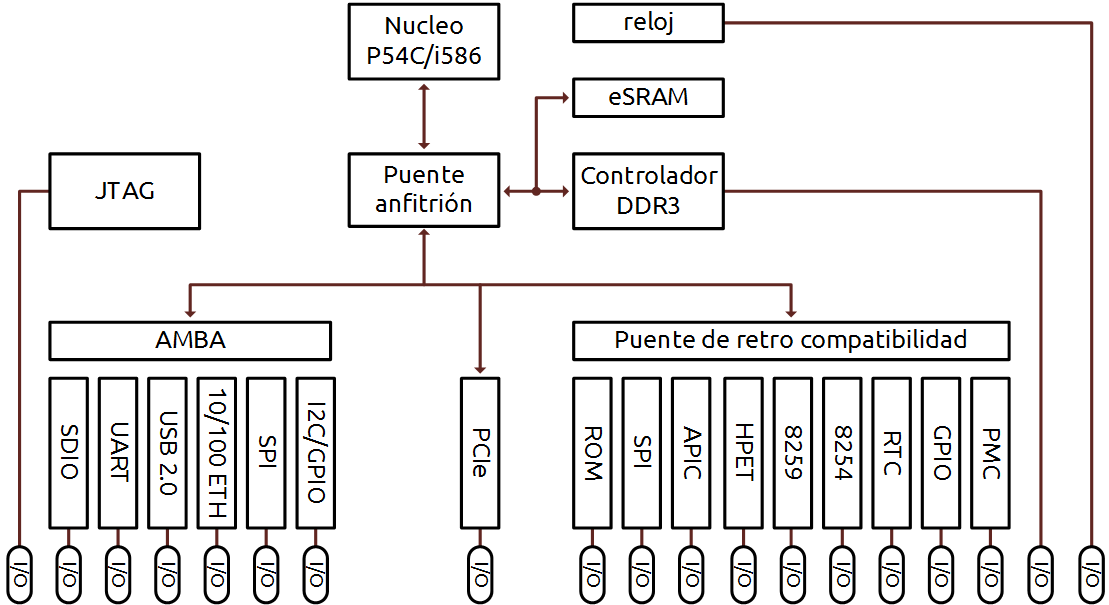
\includegraphics[scale=0.6]{figures/ch1_quark_soc.png}
	\end{center}
	\caption
		{	
			Diagrama a bloques de un dispositivo Quark\texttrademark  SoC X1000. El diseño de procesadores para ordenadores de escritorio está fuertemente relacionado con la filosofía SoC, al grado que procesadores de gama alta pueden incluir dentro del mismo silicio módulos de aceleración para el procesamiento de gráficos.
		}
	\label{fig:ch1_quark_soc}
\end{figure}

Un circuito SoC puede incluir procesadores de propósito general, bloques de memoria, aceleradores, lógica especializada, medios de interconexión y un sin número de bloques digitales que cubran las necesidades del diseño. Actualmente podemos encontrar ejemplos de sistemas electrónicos basados en SoCs prácticamente en cualquier parte de nuestro entorno, desde teléfonos celulares hasta aviones comerciales.

El concepto SoC se diversifica a razón del desarrollo de sistemas eléctricos especializados en tareas específicas. \textit{Multi Processor System on Chip} o \textit{MPSoC}\cite{chapter1:kempf:2011:multiprocessor} es un sistema SoC formado por múltiples núcleos de procesamiento o unidades funcionales. En general, un circuito MPSoC está formado por un conjunto heterogéneo de núcleos de procesamiento, y aprovecha la concurrencia entre operaciones necesarias para llevar a cabo un a tarea específica. El formato de codificación H.264/AVC\cite{chapter1:1218189} es un ejemplo popular de una aplicación que aprovecha el concepto de MPSoC, debido al número de tareas independientes que se llevan a cabo para lograr la codificación de video.

El uso de un conjunto de elementos de procesamiento heterogéneos es la arquitectura más popular para la diseño de MPSoCs. Núcleos de procesamiento dedicados a una tarea específica traen consigo beneficios de reducción de área necesaria para su tendido, eficiencia en el consumo de energía y reducción de complejidad en la validación de cada uno de ellos. Las arquitecturas MPSoC formadas por grupos de núcleos homogéneos, aunque no tan populares, han encontrado un nicho de aplicación donde el intercambio de eficiencia por flexibilidad de aplicación resulta atractivo. El uso de elementos homogéneos requiere que cada núcleo puede ser programado, desde procesadores de propósito general hasta conjuntos de unidades aritméticas capaces de ejecutar un número predeterminado de operaciones son los elementos más comunes encontrados en esta variante de MPSoC. \textit{Epiphany} es un ejemplo de un dispositivo MPSoC con núcleos de procesamiento homogéneos. Epiphany es desarrollado por la compañía Adapteva\cite{chapter1:ADAPTEVA:HOME}, el dispositivo cuenta con una arquitectura multi-núcleo escalable hasta 4,095 procesadores. Cada núcleo es un procesador de propósito general con arquitectura RISC con soporte para operaciones de punto flotante bajo el estándar IEEE de 32 bits. Epiphany utiliza un modelo de memoria compartida entre todos sus núcleos de procesamiento. La comunicación entre núcleos de un dispositivo Epiphany descansa sobre una NoC capaz de ejecutar el intercambio de mensajes entre núcleos vecinos con una latencia de 1.5 \textit{ns}. La figura \ref{ch1_epiphany_soc} muestra un diagrama a bloques de la arquitectura de Epiphany.

\begin{figure}
	\begin{center}
		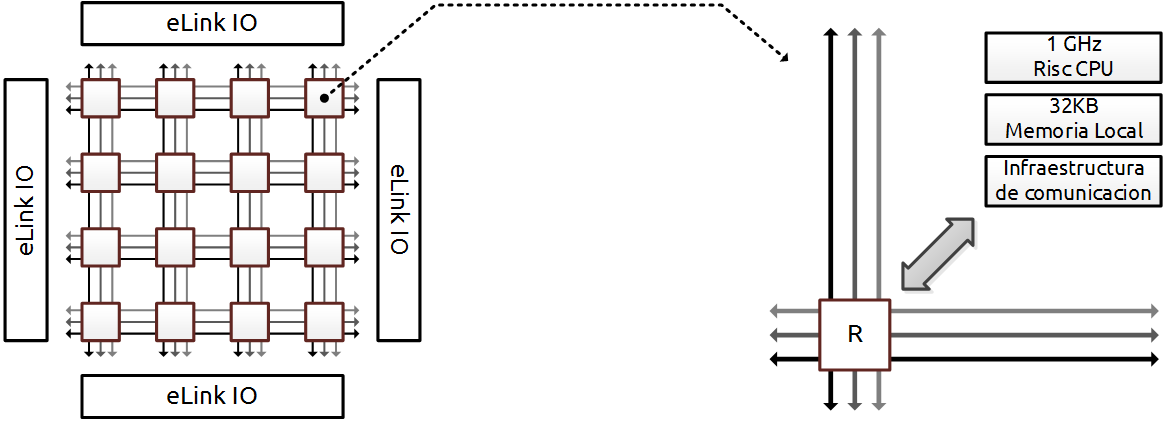
\includegraphics[scale=0.6]{figures/ch1_epiphany_soc.png}
	\end{center}
	\caption
		{	
			Diagrama a bloques de MPSoC Epiphany. Epiphany es un ejemplo de una arquitectura con núcleos de procesamiento homogéneo, algunas aplicaciones donde se a utilizado este dispositivo son: Radios definidos por software (\textit{SDR}), visión por computadora, procesamiento de sonido y video, redes neuronales y simulaciones de sistemas físicos.
		}
	\label{fig:ch1_epiphany_soc}
\end{figure}

Los siguientes trabajos presentan casos de estudio de aplicaciones específicas basadas en sistemas MPSoCs: El artículo de Tota \textit{et al.}\cite{chapter1:Tota:2009:CSN:1643330.1643337} analiza el uso de un MPSoC homogéneo como acelerador de gráficos, desde una fase de prototipado en un dispositivo reconfigurable hasta la generación de su modelo equivalente en VLSI(Very-large-scale integration); El trabajo de Jalier \textit{et al.}\cite{chapter1:Jalier:2010:HVH:1870926.1870971} ofrece una comparativa entre un MPSoC heterogéneo y una variante homogénea para la implementación de un módem para redes LTE.

La abundancia de recursos dentro de circuitos integrados no solo beneficio a dispositivos de propósito específico, gran parte de estos avances impacto en el proceso de fabricación de dispositivos reconfigurables, permitiendo incrementos en la cantidad de celdas lógicas reconfigurables y en la cantidad de bloques rígidos de propósito específico que se integran dentro de estos dispositivos. El incremento de capacidad en dispositivos reconfigurables propició la exploración del espacio de diseño con filosofía SoC/MPSoC, creando nuevas vertientes que incorporan las restricciones y propiedades físicas de los dichos dispositivos. Los términos \textit{System on Programable Chip} o \textit{SoPC}, y \textit{Programable System on-Chip} o \textit{PSoC}, se utilizan de manera frecuente para describir sistemas diseñados con filosofía SoC e implementados dentro de dispositivos reconfigurables como \textit{FPGAs}.

El rendimiento y prestaciones de un dispositivo SoC se encuentran en gran medida determinadas por la capacidad de movimiento de información entre los núcleos de procesamiento del sistema. La infraestructura de comunicación interna es un tema complejo, al cual se ha dedicado un gran esfuerzo de investigación para el desarrollo de nuevas arquitecturas más eficientes y con mejor escalabilidad. La relevancia de las estructuras de interconexión para dispositivos SoC toman un rol más preponderante en el diseño de sistemas, debido al constante incremento de núcleos que deben de comunicarse para llevar a cabo la tarea para la cual fue diseñado el dispositivo. El concepto de interconexión \textit{Network on-Chip} o \textit{NoC}, ha emergido como la solución preponderante en el desarrollo de dispositivos de próxima generación, al grado de crear filosofías de diseño alrededor de la infraestructura de interconexión y dejando en plano secundario a los núcleos funcionales del sistema. \textit{Multi Processor Network on-Chip} o \textit{MPNoC} es un ejemplo de dichas metodologías centradas en la comunicación. El concepto de red en-chip es vasto, por lo que la siguiente sección de este trabajo se presenta una breve introducción a sus fundamentos.

\section{Redes de interconexión}\label{sec:redes_de_interconexion}

Una estructura tipo bus esta formada por un grupo de lineas de transmisión de datos compartidas entre un grupo de módulos que requieren el intercambio de información. De manera ordinaria, solo dos elementos conectados a las lineas de transmisión de un bus pueden establecer un enlace durante un periodo de tiempo, dejando al resto de los módulos incomunicados de manera momentánea. La característica mencionada anteriormente hace de los buses estructuras de interconexión poco eficientes. Conforme el número de módulos que forman un sistema se incrementa, las desventajas del uso de buses como medios de interconexión se hacen más notorias. Buses jerárquicos\cite{chapter1:100306} y buses segmentados\cite{chapter1:797400} son algunos de los ejemplos de modificaciones estructurales que sufrieron los buses para mejorar su desempeño, sin embargo el incremento en las frecuencias de operación en silicio y un aumento en el número de módulos dentro de un circuito SoC orillo a la búsqueda de nuevas estructuras para la transmisión de datos.

Diseños electrónicos complejos integrados en un solo empaquetado migraron del uso de buses como infraestructura de comunicación a redes mas complejas para su interconexión. Una \emph{red de interconexión} puede definirse como un \emph{sistema programable para el transporte de información entre módulos o nodos, donde las lineas físicas de transporte de información son compartidas entre todos los miembros de la red}. La principal característica que distingue a una red de interconexión entre otros medios de enlace es su modelo general de operación: Una red trabaja bajo el concepto de intercambio de mensajes entre nodos miembro; Si un nodo desea enviar un mensaje a un nodo vecino, este debe de entregar el mensaje a la red y esta a su vez se encargará de que dicho mensaje sea entregado a su destinatario. Otros medios de enlace, como lineas de comunicación dedicadas, se limitan a operar como simples medios físicos para el intercambio de datos.

Los términos \textit{sistema} y \textit{programable} que forman parte de la definición de red de interconexión, proveen de elementos extra para diferenciar este concepto de otros medios de enlace. Una red de interconexión se considera un sistema porque está formado de varios componentes como: buffers, canales de transmisión, lógica de control y switches. El término programable indica la capacidad de la red para crear diferentes conexiones entre nodos, utilizando un conjunto de recursos limitados pero compartidos para la transmisión de datos desde cualquier miembro del sistema.

Las redes de interconexión ofrecen grandes beneficios en comparación con otras estructuras tradicionales, por ejemplo, la figura \ref{fig:ch1_enlaces_dedicados} presenta dos estructuras para interconectar seis nodos. A la izquierda se presenta el enlace de todos los miembros del sistema mediante lineas de conexión dedicadas entre cada uno de los nodos. Se requieren de 30 líneas de transporte de datos para conectar cada nodo con sus vecinos. En contraparte, la red de interconexión a la derecha en la figura \ref{fig:ch1_enlaces_dedicados} requiere solo de $1/5$ de los recursos requeridos por la primera estructura. 

\begin{figure}
	\begin{center}
		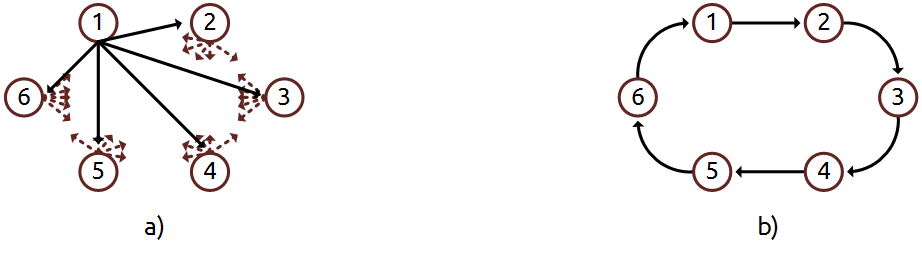
\includegraphics[scale=0.7]{figures/ch1_enlaces_dedicados.png}
	\end{center}
	\caption
		{	
			a) Enlace de 6 nodos mediante líneas de comunicación dedicadas entre terminales. b) Enlace de 6 nodos mediante una red de interconexión en forma de anillo.
		}
	\label{fig:ch1_enlaces_dedicados}
\end{figure}

Las redes de interconexión no solo ofrecen una reducción en la cantidad de recursos para el enlace entre nodos, imagine que cada nodo de las estructuras presentadas en la figura \ref{fig:ch1_enlaces_dedicados} requiere transmitir un mensaje a cada otro nodo en intervalos de 100 ciclos de reloj. En el modelo con enlaces dedicados, cada enlace estará ocupado solo durante el 1\% del tiempo de operación del sistema. El enlace por medio de una red de interconexión con forma de anillo tendrá un factor de trabajo de entre 12\% y 15\% dependiendo de los detalles de organización de la red.

El concepto de red de interconexión y sus fundamentos pueden aplicarse a diferentes escalas: desde redes para la interconexión de computadoras dentro de un edificio, denominadas \textit{redes de área local} o \textit{LAN}; Redes de conexión entre circuitos de un sistema electrónico, o hasta redes de interconexión de módulos dentro de un SoC, denominadas \textit{Networks on-Chip} o \textit{NoC}. Este último término, traducido al español como \textit{Redes en-Chip}, es uno de los fundamentos de este trabajo, y a partir de este punto del documento los términos red de interconexión y \textit{NoC} se utilizaran de manera indistinta. En el trabajo\cite{chapter1:Bjerregaard:2006:SRP:1132952.1132953} se encuentra un recopilado de el espacio de diseño y campos de investigación en NoCs.





\section{Conceptos básicos de NoCs}\label{sec:conceptos_basicos_de_nocs}

Una NoC ofrece el servicio de transporte de mensajes entre nodos miembro de una red. De manera general, todo nodo de una red en-chip está formado por tres elementos principales: un elemento de procesamiento, una interfaz de red y un \textit{router}. El elemento de procesamiento representa una unidad funcional, puede ser un procesador de propósito general, lógica para la ejecución de una operación específica o un elemento de almacenamiento. El router forma parte de la infraestructura de la red, su tarea principal consiste en la recepción, calculo de ruta y reenvío de paquetes en dirección a un nodo destino. El término \textit{router} se traduce al español como encaminador o enrutador. 

La interfaz de red consiste en una etapa de lógica de acoplamiento entre el elemento de procesamiento y el router de un nodo. La interfaz de red traduce paquetes de datos a un formato de trabajo para el elemento de procesamiento, de igual forma, la interfaz se encarga de tomar los resultados del elemento de procesamiento y empaquetarlos de manera que puedan ser transportados a través de la NoC. La figura \ref{fig:ch1_nodo_simple} muestra la estructura de un nodo de red estándar. Utilizaremos el término \textit{canal} para referirnos a un conjunto de líneas de transporte de datos que enlazan a un nodo con un vecino inmediato.

\begin{figure}
	\begin{center}
		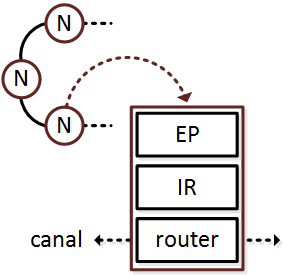
\includegraphics[scale=0.8]{figures/ch1_nodo_simple.png}
	\end{center}
	\caption
		{	
			Nodo de red: N representa un nodo de red, EP simboliza un elemento de procesamiento e IR a una interfaz de red. \textit{Canal} es el término utilizado para referirse a las líneas físicas de transmisión de datos entre un nodo y uno de sus vecinos de la red.Los nodos miembros de una red pueden ser heterogéneos. No existe un modelo único de interfaz de red, ya que diferentes tipos de elementos de procesamiento requieren la presentación de los datos de trabajo en diferentes formatos.
		}
	\label{fig:ch1_nodo_simple}
\end{figure}

Una red en-chip está definida por 3 características principales: topología, algoritmo de planificación de ruta y esquema de control de flujo de datos. Topología se le llama al patrón de distribución de nodos y canales a través de red. El término \textit{grado del nodo} define el número de canales que comunican un nodo con sus vecinos. Los nodos del segmento de red mostrados en la figura \ref{fig:ch1_nodo_simple} tienen un \textit{grado 2}, es decir un canal por cada vecino.

Un mensaje puede tomar diferentes vías a través de la red para llegar a su destino. La selección de uno de los múltiples caminos para el transporte de información está a cargo del algoritmo de planificación de ruta. Una ruta está formada por el conjunto de nodos y canales que un mensaje deberá de cruzar antes de llegar a su destino. Una práctica común es el referirse como \textit{número de saltos} a la cantidad de routers que un mensaje debe visitar antes de llegar a su destino. Un buen algoritmo de planificación de ruta busca reducir el número de saltos necesarios para entregar un mensaje a su destinatario mientras mantiene a todos los canales de la red ocupados. Si el algoritmo de planificación tiende a saturar algunas rutas de la red, mientras otras se encuentran en estado de reposo, se dice que el algoritmo propicia \textit{desbalances de carga}. Dentro del argot de redes en-chip, suelen utilizarse los términos \textit{ruteo} o \textit{encaminamiento} para referirse a la acción del cálculo de ruta que tomará un mensaje a través de la red, en este documento utilizaremos cualquiera de estos términos de manera indistinta.

El control de flujo de datos son políticas aplicadas en cada router e interfaz de red para administrar el uso de recursos como: canales, puertos de entrada y salida, buffers, y cualquier elemento compartido para la transmisión de mensajes. Los mecanismos de control de flujo se aplican en diferentes elementos de la red, pero en conjunto, buscan reducir el tiempo que tarda un mensaje en alcanzar a su destinatario y evitar la pérdida de mensajes durante su traslado.





\subsection{Topología}

La topología de una NoC define el arreglo de conexiones entre nodos y canales que forman la red. La topología es análoga al mapa de una carretera, donde cada ciudad o poblado representa un nodo de la red y los tramos de camino representan los canales entre nodos. La figura \ref{fig:ch1_topologia} muestra una red con topología tipo torus y una red de topología tipo anillo, ambos ejemplos se consideran \textit{redes directas}, ya que cada router de la red está conectado de manera directa con un elemento de procesamiento. En caso que uno o más routers de la red no estén ligados de manera directa a un elemento de procesamiento, se considera a dicha red como \textit{indirecta}.

\begin{figure}
	\begin{center}
		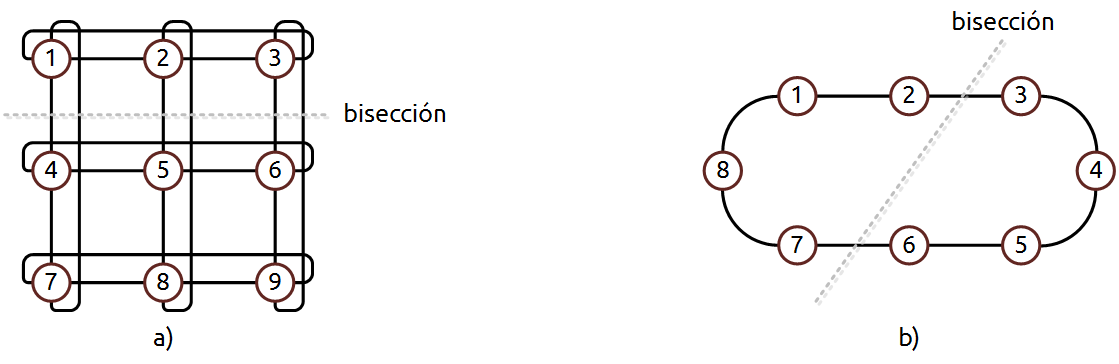
\includegraphics[scale=0.7]{figures/ch1_topologia.png}
	\end{center}
	\caption
		{	
			a) Topología tipo torus de 9 nodos. b) Topología tipo anillo con 8 nodos. Cada línea de interconexión en el diagrama representa dos canales en direcciones opuestas, por ejemplo, la línea entre los nodos 1 y 2 de la red tipo anillo representa: un canal saliente del nodo 1 en dirección del nodo número 2 y un canal saliente del nodo número 2 con dirección del nodo 1.
		}
	\label{fig:ch1_topologia}
\end{figure}

La topología tiene un alto impacto en el rendimiento de una NoC, por ejemplo, el máximo \textit{ancho de banda} (Tasa máxima de transferencia de datos a través de un segmento de la red, la unidad de transferencia de datos utilizada para tasar el ancho de banda es $bits/sec$.) que puede ejercer una red está determinado por el ancho de banda de bisección. La bisección de una NoC conciste en el grupo de canales que son seccionados por una línea imaginaria que divide la red en dos segmentos. La figura \ref{fig:ch1_topologia} destaca la bisección de ambas topologías ilustradas.

Utilicemos las dos redes de la figura \ref{fig:ch1_topologia} como ejemplo para evaluar cómo la topología repercute en el rendimiento de una NoC. Los parámetros base para ambos ejemplos son los siguientes: Ambas redes tienen una frecuencia de operación de 300 MHz (periodo = 3.33 ns), el ancho de canal para la red con topología torus es de 32 bits mientras que para la red de topología tipo anillo es de 64 bits. Es importante notar que en la figura \ref{fig:ch1_topologia} cada linea que conecta dos nodos representa dos canales en direcciones opuestas, es decir, desde el punto de vista de un nodo cada línea representa un canal saliente y un canal ingresando a el.

El \textit{ancho de banda de bisección} para la red torus se calcula como el producto entre el número de canales que cruza la bisección(12), el ancho de palabra de cada canal(32 bits) y la frecuencia de operación de la red (300 MHz). La ejecución del producto anterior da como resultado un total de 115.2 $Gbits/s$. El ancho de banda en la bisección de la topología tipo anillo se calcula de manera similar, sustituyendo los canales en bisección(4) y el ancho de cada canal(64 bits). La máxima tasa de transferencia en la bisección para la red anillo es de 76.8 $Gbits/s$. En este caso particular, la red torus ofrece 1.5x veces mayor capacidad de transferencia de datos en comparación con la red tipo anillo.

La tasa máxima de transferencia de una red no es único indicador de rendimiento. Retomemos el ejemplo anterior definiendo 4,096 bits como el tamaño de los mensajes a transmitir a través de la red. Definamos el termino \textit{latencia promedio} como el tiempo promedio que tarda un mensaje en ser entregado a su destinatario. Para el cálculo de la latencia promedio, es necesario la selección de un \textit{patrón de trafico}, el cual es un modelo de probabilidad y frecuencia de comunicación entre nodos de una red. Los patrones pueden ser generados de manera artificial o a partir de la captura del esquema de comunicación entre nodos de un sistema preexistente. En este ejemplo utilizaremos un patrón aleatorio, donde todos los nodos de la red tienen la misma probabilidad de ser electos como destino de un mensaje. En el trabajo\cite{chapter1:Bahn09ageneric}, presentado por Bahn y Bagherzadeh, se aborda la generación de patrones de prueba para redes en-chip. Además, es necesario definir el término \textit{distancia promedio}, el cual representa el número de saltos en promedio que un paquete debe de llevar a cabo para alcanzar cualquier nodo de la red. Para la red torus la distancia promedio es de 2 saltos, mientras que en la red anillo la distancia promedio también es de 2 saltos. Supongamos que para ambas redes, el tiempo promedio para ejecutar un salto entre dos nodos es de 9.99 ns (3 ciclos de reloj).

Mensajes de 4,096 bits de longitud, con canales de 32 y 64 bits de ancho de palabra, hacen necesario la \textit{serialización} de los mensajes, es decir, la división de estos en bloques de tamaño igual al ancho de palabra del canal. El proceso de división de un mensaje trae consigo una penalización de latencia equivalente al tiempo que se requiere para extraer un fragmento del mensaje original. A esta penalización se le denomina \textit{latencia de serialización}. Supongamos que la latencia de serialización para ambas tipologías es igual a un ciclo de reloj por bloque.

El tiempo promedio de transporte de un mensaje en la red de topología torus es igual a la latencia de serialización del mensaje en fragmentos de 32 bits ($4,096/32 = 128$ ciclos), más el tiempo requerido para cubrir la distancia promedio entre nodos de la red ($9.99ns * 2 = 19.98ns$), es decir la \textit{latencia promedio} para esta red es de 2983.68 ns para el transporte de los 128 paquetes que conforman un mensaje de 4,096 bits. Para la topología tipo anillo, que cuenta con canales de 64 bits, la latencia de serialización es de 213.12 ns. Si a esta última cifra agregamos el tiempo necesario para llevar a cabo los dos saltos promedios de la red tenemos una \textit{latencia promedio} total de 1491.82 ns por mensaje.

Este último resultado presenta a la topología tipo anillo como la infraestructura que ofrece la menor latencia para la entrega de mensajes a través de la red, aun cuando la red de topología torus ofrece un mayor ancho de banda para la transmisión de datos. La selección de topología depende de las características y requerimientos de la aplicación además de las restricciones físicas del dispositivo que pueden restringir el uso de ciertas topologías.

Sadawarte\cite{chapter1:Sadawarte:2011:CSS:1947940.1947992} presenta  un compilado de fuentes de información respecto a las topologías más comunes utilizadas en redes en-chip, este documento es un gran punto de inicio para profundizar en el tema.




\subsection{Planificación de ruta}

La ruta o camino entre dos nodos de la red se representa mediante un conjunto ordenado de canales $P=\{c1, c2,\dots,c_{n}\}$. Cada canal $c_{n}$ representa un punto de entrada y uno de salida. El punto de salida del canal $c_{n}$ es el punto de entrada del canal $c_{n+1}$. Físicamente, la topología provee de múltiples rutas $P$ para la transmisión de mensajes entre dos nodos de la red, sin embargo, es tarea del algoritmo de planificación de ruta la selección del camino para cada transferencia de datos. Los términos \textit{routing}, \textit{ruteo} o encaminamiento se utilizan de manera indistinta para hacer referencia al algoritmo de planificación de ruta de una NoC.

Un algoritmo de ruteo eficiente procura la reducción del número de saltos necesarios para la transferencia de un mensaje, a la vez que procura evitar la saturación de un conjunto reducido de canales de la red. La saturación de ciertos canales mientras rutas alternas se encuentran disponibles se denomina \textit{desbalance de carga}.

Es una práctica común nombrar a los nodos de una red mediante coordenadas que reflejen su posición respecto a sus vecinos. La figura \ref{fig:ch1_ruteo} muestra redes con topologías tipo \textit{malla}, los identificadores asignados a cada nodo de estas redes consta de una tupla \{x,y\} que representa su posición en coordenadas de un plano cartesiano. Los algoritmos ordenados por dimensión se caracterizan por realizar avances en una dirección a la vez, por ejemplo: la transferencia entre los nodos \{1,0\} y \{0,2\} en la figura \ref{fig:ch1_ruteo} (a) presenta dos rutas posibles: la primera ruta visita los nodos \{1,1\} y \{1,2\}, ejecutando todos los saltos necesarios en la dirección \textit{x} antes de entregar su mensaje mediante un último salto en la dirección \textit{y}; De manera contraria, la ruta con saltos a los nodos \{0,0\} y \{0,1\}, lleva a cabo en primer lugar un salto en la dirección \textit{y}.

El algoritmo de \textit{ruteo XY}\cite{chapter1:Priyanka:2013:IJCA} es un ejemplo popular de planificación de ruta ordenada por dimensión. Este tipo de algoritmos tienden a ser sencillos y ofrecer \textit{rutas mínimas} para la entrega de mensajes. \textit{Ruta mínima} se denomina a un camino que requiere el mínimo de saltos para alcanzar su objetivo, las dos rutas presentes en la figura \ref{fig:ch1_ruteo} (a) son rutas mínimas entre los nodos \{1,0\} y \{0,2\}.

\begin{figure}
	\begin{center}
		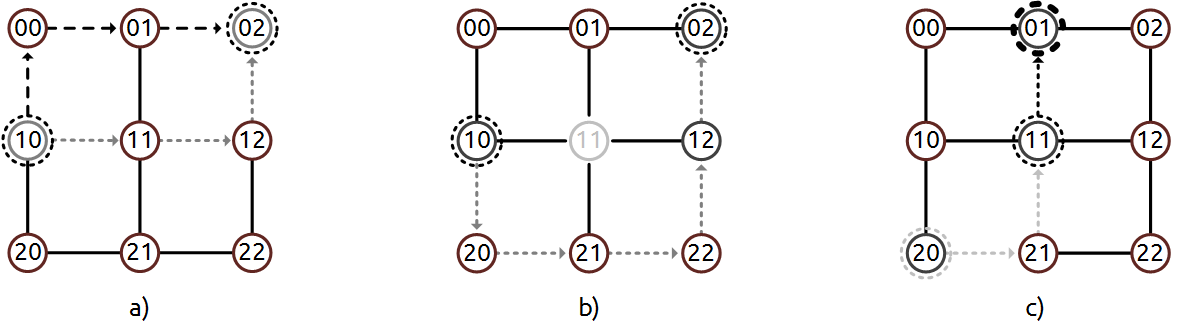
\includegraphics[scale=0.7]{figures/ch1_ruteo.png}
	\end{center}
	\caption
		{	
			Tres instancias de una red con topología tipo malla o \textit{mesh}. Las direcciones para cada nodo de red se forman de una dupla de coordenadas \textit{\{x|y\}}. a) Rutas trazadas mediante algoritmos de ordenamiento dimensional. b) planificación de una ruta no mínima entre dos nodos de la red. c) Desbalance de carga en la red, el canal que vincula a los nodos \{1,1\} y \{0,1\}.
		}
	\label{fig:ch1_ruteo}
\end{figure}

Los algoritmos ordenados por dimensiones tienen la desventaja de propiciar la saturación de canales en la red. Por ejemplo, en la figura \ref{fig:ch1_ruteo} (c) el canal entre los nodos \{0,1\} y \{1,1\} es utilizado en todas las rutas con destino al nodo \{0,1\} que parten desde los nodos en las filas 1 y 2 de la red. Conforme aumente la demanda de transferencia de mensajes al nodo \{0,1\}, el ancho de banda disponible en los canales de acceso desde la dirección \textit{y-} se reduce, mientras la latencia de transferencia de mensajes aumenta. Algoritmos que pueden seleccionar rutas no mínimas como la trazada en la figura \ref{fig:ch1_ruteo} (b) tienden a reducir el problema del balanceo de carga en la red, sin embargo suelen ser más complejos y pueden generar bloqueos en la red en caso de no estar verificados de manera exhaustiva. Los algoritmos con capacidad de generar rutas tanto mínimas como no mínimas se denominan \textit{algoritmos adaptativos}. Los algoritmos adaptativos dan flexibilidad a la red, ofreciendo un mejor balance en la carga de sus canales y ofreciendo rutas alternas en caso que algunos de los nodo miembro no se encuentre disponible para reenviar un mensaje en dirección de su destino, sin embargo el uso de rutas más largas entre nodos aumenta la latencia promedio para la entrega de los mensajes, además de requerir hardware más complejo para la toma de decisiones. Existen algoritmos exclusivos para su uso en conjunto con topologías específicas, por ejemplo, el algoritmo aEqualized\cite{chapter1:5090764} está diseñado para su uso exclusivo con topologías tipo spidergon.




\subsection{Estructura de mensajes}

Hasta este momento se ha utilizado el \textit{mensaje} como unidad básica de transporte de información a través de la red sin embargo la mayoría de redes de interconexión requieren descomponen un mensaje en segmentos de tamaño igual al ancho de sus canales de enlace. Un mensaje puede tener una longitud arbitraria y dependiente de la aplicación, por ejemplo para un sistema de procesamiento de imágenes un mensaje puede contener la información de todos los píxeles capturados por una cámara, mientras para una red distribuida de sensores, el mensaje puede tener la longitud necesaria para transmitir una lectura de temperatura. La diferencia entre tamaños de mensaje en las aplicaciones anteriormente descrita puede estar entre varios megabytes de información a unos cuantos bytes.

Para facilitar el manejo de información a través de la red los mensaje son fracturados en \textit{paquetes}. Un paquete contiene una sección de la información que forma un mensaje, y es la unidad básica para las operaciones de control y transferencia de datos entre routers. Cuando un router de la red asigna recursos para una transacción, la asignación tendrá una duración equivalente al tiempo necesario para movilizar al siguiente salto  todos los datos que forman un paquete. A todo paquete liberado a la red se le anexa información de control para que este se capaz de navegar a su destino, y para poder reconstruir un mensaje una vez que todos los paquetes hayan sido capturados. Los paquetes deben de tener una restricción sobre el tamaño máximo que pueden alcanzar, de manera que se pueda tener un estimado en la cantidad de recursos y tiempo que se le asigna a cada paquete en la red. Los paquetes de un mensaje puede contener información de control, datos de trabajo o una combinación de ambos.

Los paquetes a su vez se dividen en \textit{flits}(control flow digit) o dígitos de control de flujo. El flit es la unidad atómica para la asignación de espacio en buffer, por lo que todos los routers de la NoC deben de proveer espacio al menos para un flit en transito. Esta ultima regla no aplica si el router de red utiliza una estrategia de control de flujo sin almacenamiento temporal. Las estructura de un paquete segmentado incluye un \textit{flit de cabecera}, uno o más \textit{flits de datos} y un \textit{flit de terminación}. El flit de cabecera de manera general no contiene parte de la información del mensaje, en su lugar, este flit acarrea la información necesaria para abrirse paso a través de la red hasta su destino. Por ejemplo, un flit de cabecera puede contener la dirección del nodo destino del mensaje. Los flits de datos generalmente cargan un segmento del mensaje enviado a través de la red, sin embargo, también pueden contener algunos bits de control para identificarse como flits de datos. Finalmente, un flit de terminación anuncia el final de un paquete. El flit de terminación es utilizado cuando los paquetes de la red pueden tener un número no predeterminado de flits de datos.

En caso de que el tamaño en bits de un flit sea superior al número de líneas físicas que conforman un canal, será necesario dividir los flits de un paquete en \textit{phits} o \textit{unidades físicas}. El phit es el máximo de información que se puede transferir de un nodo a otro en un solo ciclo de reloj. La figura \ref{fig:ch1_jerarquia_mensajes} muestra la descomposición de un mensaje en unidades de dimensiones inferiores.

\begin{figure}
	\begin{center}
		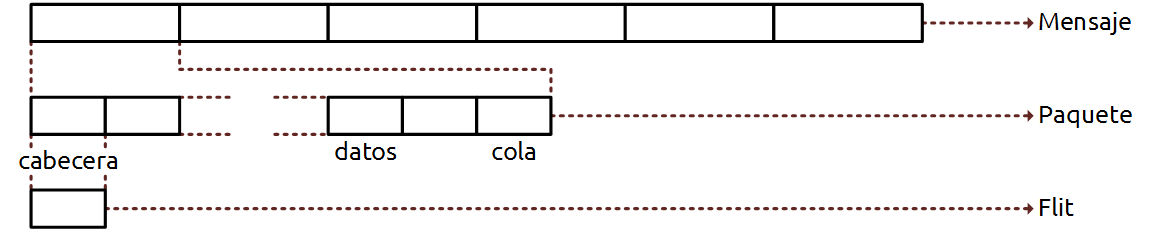
\includegraphics[scale=0.7]{figures/ch1_jerarquia_mensajes.png}
	\end{center}
	\caption
		{	
			Estructura de un mensaje. La división de un mensaje puede ser física o lógica, dependiendo del contexto de manejo en el cual se esté procesando la información. En la figura no se muestra la división de flits en phits.  
		}
	\label{fig:ch1_jerarquia_mensajes}
\end{figure}


\subsection{Control de flujo}

El control de flujo de datos de una NoC establece las políticas para la asignación de recursos que permitirán a los paquete avanzar a través de la red. Las políticas de control de flujo se encargan de administrar los canales entre nodos y los buffers internos de cada router. Los buffers de un router permiten almacenar de manera temporal los paquetes que, por algún motivo, no pueden continuar de manera inmediata su camino. 

El funcionamiento de los buffer dentro de un nodo, siguiendo la analogía con una carretera, representan un carril exclusivo para incorporarse a otra intersección. Si un automóvil, que en esta analogía representa un paquete, quiere incorporarse a una intersección saturada, este deberá esperar su turno para ingresar a carril deseado. Durante el tiempo de espera otro automóvil que desea continuar por el camino principal llega a la intersección, este último automóvil no puede continuar su trayecto debido a que el automóvil esperando a incorporarse a la intersección se encuentra bloqueando su paso. Agregando un carril exclusivo para los automóviles que desean dejar el camino principal se previenen posibles bloqueos, permitiendo el avance de automóviles sin obstáculos en las intersecciones.

Las políticas de control de flujo definen el avance de un paquete entre nodos y dentro de sus correspondientes routers. El control de avance entre nodos puede pensarse como semáforos, controlando cuándo es momento para que un automóvil tenga acceso al siguiente segmento de carretera.

Una buena política de control de flujo procura evitar el bloqueo de paquetes en tránsito debido a la falta de recursos, en especial en el caso que existan recursos disponibles en otras áreas de la red. De igual manera, el control de flujo debe evitar situaciones donde varios paquetes en circulación generen un \textit{punto muerto} o \textit{deadlock}, donde el avance de estos paquetes sea imposible debido a dependencias circulares de recursos entre ellos. Otra situación que el control de flujo debe evitar es la creación de \textit{livelocks} o \textit{paquetes errantes}, en esta situación un paquete en la red no recibe los recursos adecuados para alcanzar su destino y por consiguiente se encuentra vagando entre nodos de manera permanente. Estos dos últimos escenarios, \textit{deadlock} y \textit{livelock}, son resultado de políticas injustas al momento de asignar recursos entre paquetes compitiendo por ellos. La figura \ref{fig:ch1_deadlock} presenta una situación de deadlock en una red en-chip. El control de flujo puede verse como un problema de asignación de recursos o como una tarea de resolución de conflictos entre paquetes disputando estos recursos.

\begin{figure}
	\begin{center}
		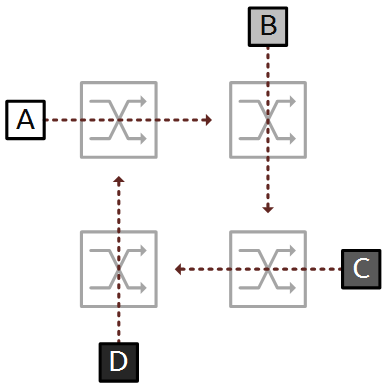
\includegraphics[scale=0.7]{figures/ch1_deadlock.png}
	\end{center}
	\caption
		{	
			Deadlock en una NoC. En este ejemplo El paquete A espera los recursos reservados por el paquete B, que a su vez espera los recursos asignados al paquete C, el cual, no puede avanzar por el bloqueo de recursos causado por el paquete D, el cual cierra la \textit{dependencia circular} esperando los recursos del paquete A.
		}
	\label{fig:ch1_deadlock}
\end{figure}

El mecanismo más sencillo de control de flujo se denomina \textit{bufferless}, el término se deriva de la aplicación de políticas de gestión de recursos que no consideran la disponibilidad de buffers en los diferentes nodos de la red. El manejo de disputas por recursos entre paquetes es solucionada por medio de el \textit{descarte} del paquete no ganador, o mediante el \textit{reenvío} del paquete por cualquier canal de salida que se encuentre disponible en ese momento, inclusive, si el canal disponible envía al paquete en la dirección opuesta de su destino. Estos dos mecanismo de resolución de conflictos pueden ser referidos por los términos \textit{drop} o \textit{misroute} respectivamente. La figura \ref{fig:ch1_bufferless} ejemplifica las dos estrategias utilizadas con un mecanismo bufferless de control de flujo.

\begin{figure}
	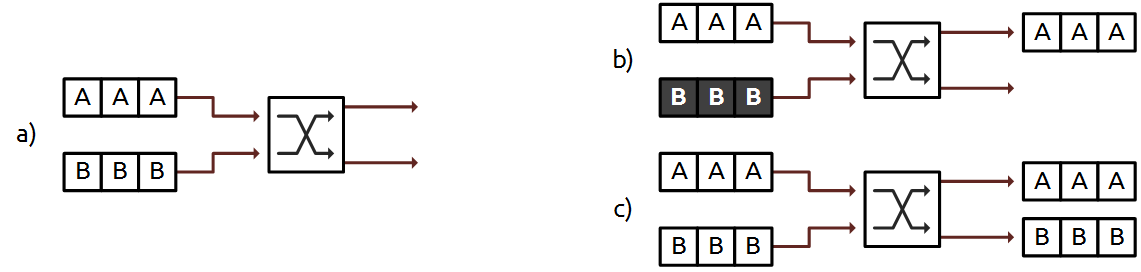
\includegraphics[width=\linewidth]{figures/ch1_bufferless.png}
	\caption
		{	
			Control de flujo bufferless. a) Dos paquetes llegan al router solicitando el puerto de salida superior. b) Bajo una estrategia de \textit{descarte} el paquete A gana control de los recursos para avanzar mientras el paquete B es desechado. b) En una estrategia de \textit{reenvío} el paquete B en lugar de ser descartado se le da salida a través del puerto disponible.
		}
	\label{fig:ch1_bufferless}
\end{figure}

\textit{Conmutación de circuitos} o \textit{circuit switching} es una estrategia de control de flujo con mayor compromiso respecto a la fiabilidad de la entrega de mensajes entre nodos. Este mecanismo inicia toda transmisión con el envío de un paquete de cabecera. Los paquetes de cabecera contienen información de encaminamiento de manera exclusiva. La cabecera reserva el uso de los recursos que ha utilizado durante su avance a través de la red, una vez alcanzado su destino, todos los recursos reservados forman un \textit{túnel} entre el nodo origen y el nodo destino. Ningún paquete o flit de datos entrara a la red a menos que el túnel, también llamado \textit{circuito}, está formado de manera satisfactoria. Se puede llevar a cabo cualquier número de transacciones entre los nodos enlazados siempre y cuando el circuito entre nodos se encuentre activo. Una vez finalizada la transmisión de datos, uno de los nodos enlazados debe de emitir un paquete para la liberación de los recursos reservados. Una gran desventaja del uso de esta estrategia es el bloqueo de recursos durante la vida de un enlace entre nodos, los recursos reservados no pueden ser utilizados por ningún otro paquete hasta que sean liberados. La conmutación de circuitos requiere sólo de asegurar el almacenamiento temporal para un flit.

La figura \ref{fig:ch1_circuit_switching} muestra una transacción estándar en una red que hace uso del esquema de conmutación de circuitos, la transmisión inicia con el envío de un flit de cabecera, este tarda 4 ciclos de reloj para llegar al nodo destino de la transmisión. El nodo destino procesa la petición de establecimiento de circuito durante el ciclo 4 y en el siguiente flanco positivo de la señal de sincronización libera un señal de confirmación de establecimiento de enlace. Durante el noveno ciclo de operación, el nodo origen recibe la confirmación de la formación del circuito con el nodo destino, a partir de este momento se puede iniciar con la transferencia de datos. La transferencia de datos en la figura \ref{fig:ch1_circuit_switching} se lleva a cabo en ráfagas independientes, el envió de datos puede llevarse a cabo bajo cualquier patrón de intervalos de transferencia e inactividad durante el tiempo que se mantenga el enlace entre nodos. Finalmente el nodo origen libera un flit de terminación que libera los recursos del circuito conforme avanza en dirección del nodo destino.

\begin{figure}
	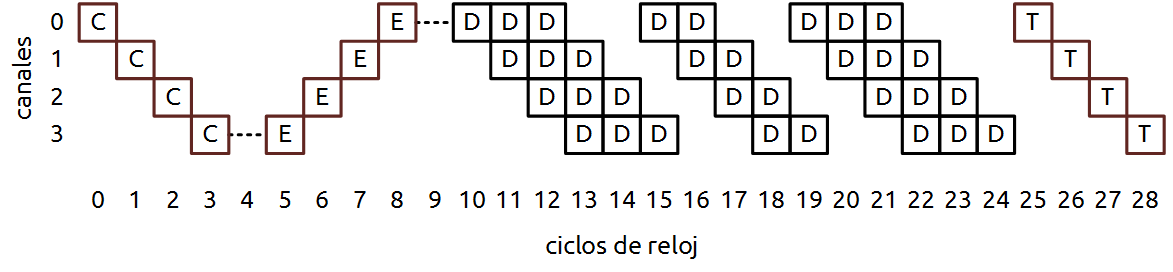
\includegraphics[width=\linewidth]{figures/ch1_circuit_switching.png}
	\caption
		{	
			Secuencia de transmisión de datos mediante conmutación de circuitos. El identificador \textit{C} representa la cabecera de un paquete, \textit{E} representa un mensaje de confirmación de creación de enlace, \textit{D} representa la carga efectiva de datos de un paquete y \textit{T} representa el final de un paquete.
		}
	\label{fig:ch1_circuit_switching}
\end{figure}

El esquema más popular para el control de flujo en la actualidad es la \textit{conmutación de paquetes} o \textit{packet switching}. Esta técnica obtiene ganancias en rendimiento mediante el almacenaje de paquetes previo a la asignación de recursos, desacoplando de manera efectiva el proceso de transmisión de datos y de solicitud de canales de salida. La conmutación de paquetes es un concepto del cual se derivan diferentes esquemas de control de flujo, cada esquema se diferencia por la granularidad de sus buffers y por el mínimo de almacenamiento requerido para permitir el salto de datos entre nodos de la red. Los esquemas más populares de conmutación de paquetes son: \textit{store \& forward}, \textit{cut-through}, y \textit{wormhole}.

Los esquemas \textit{store \& forward} y \textit{cut-through}, requieren garantizar al menos el espacio suficiente para un paquete completo en el nodo receptor antes de proceder con el reenvío de un mensaje. La principal diferencia entre estos dos esquemas radica en la condición para el inicio de reenvío de paquetes al siguiente nodo, en store \& forward se requiere tener almacenado en su totalidad un paquete antes de poder reenviarlo al siguiente salto, mientras que en cut-through, es posible reenviar de manera inmediata parte de un paquete al siguiente nodo siempre y cuando se asegure tener espacio suficiente para recibir el paquete completo en el siguiente router. La figura \ref{fig:ch1_store_cut}(a) muestra una transacción bajo el esquema store \& forward, en este ejemplo cada salto entre nodos tiene una duración de 5 ciclos de reloj, debido a que cada paquete debe ser almacenado en su totalidad dentro de un buffer de manera previa a su reenvío a través de un puerto de salida.  b) y c) de la figura \ref{fig:ch1_store_cut} muestran el comportamiento de un router con control de flujo cut-through bajo dos escenarios. El primer escenario, ilustrado por la figura \ref{fig:ch1_store_cut} (b), muestra una red en estado de reposo, en este caso la transmisión entre nodos inicia de manera inmediata, retransmitiendo en primer lugar el flit de cabecera al siguiente salto de la ruta. En la figura \ref{fig:ch1_store_cut} (c), el salto entre los canales 1 y 2 presenta un bloqueo temporal, donde el nodo que maneja la salida del canal 1 debe de esperar durante 3 ciclos de reloj para que el nodo receptor libere suficiente espacio para la recepción de todos los flits del paquete. Este segundo escenario es una muestra del comportamiento de la red bajo cargas de trabajo pesadas.

\begin{figure}
	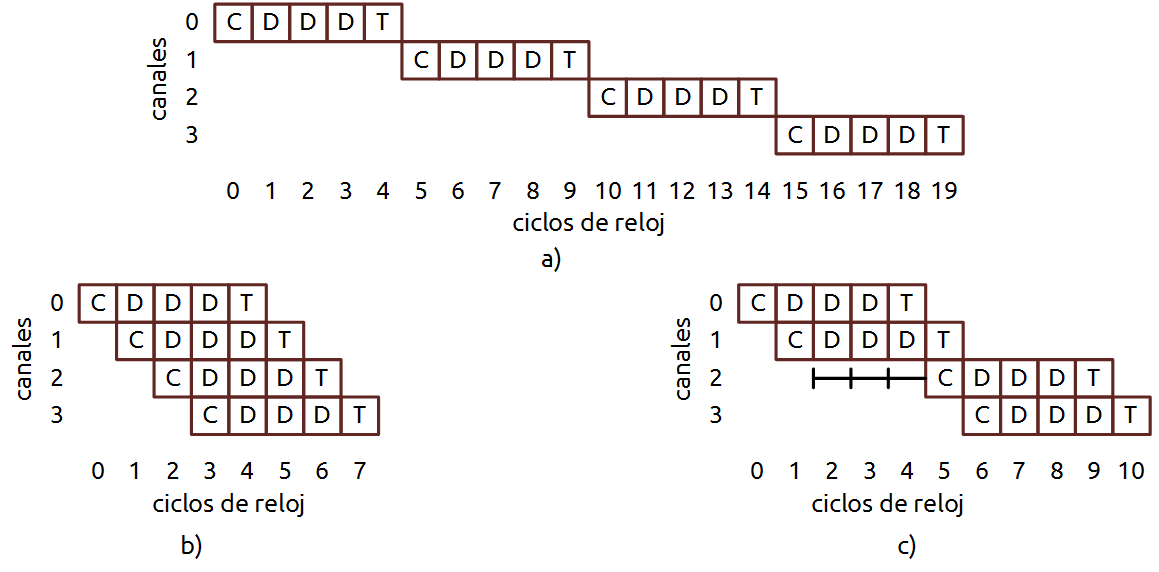
\includegraphics[width=\linewidth]{figures/ch1_store_cut.png}
	\caption
		{	
			Transferencias con controles de flujo basados en granularidad de paquete. a) Transferencia \textit{store \& forward}, antes de ejecutar el próximo salto en la red, todo el paquete debe de estar almacenado en el router actual. b) Bajo el esquema \textit{cut-through} no es necesario la espera de recepción de todos los flits de un paquete, tan pronto se cuente con espacio suficiente en el siguiente router se puede iniciar la transferencia de flits. c) En caso de no contar con espacio suficiente en el siguiente salto, los flits de un paquete se almacena en buffer sin riesgo de pérdidas, al momento de asegurar recursos en el siguiente router se reanuda la transferencia. 
		}
	\label{fig:ch1_store_cut}
\end{figure}

\textit{Wormhole} trabaja a nivel de granularidad de flits, por lo que demanda al menos tener seguro el espacio suficiente para recibir un flit antes de continuar la transferencia de un paquete. La figura \ref{fig:ch1_wormhole} muestra el desenvolvimiento de una operación de tránsito de paquetes a través de un router con control de flujo tipo wormhole. El buffer del router mostrado en la figura \ref{fig:ch1_wormhole} tiene una capacidad de almacenamiento de 2 flits. Durante el primer ciclo de captura, figura \ref{fig:ch1_wormhole} (a), la cabecera del paquete ingresa al router y de manera inmediata le sigue el primer flit de datos. Hasta el ciclo mostrado en la figura \ref{fig:ch1_wormhole} (c), no ha habido desplazamiento alguno de flits fuera del router. La lógica de control y planeación de ruta utilizan la información del flit de cabecera, recibido un ciclo previo, para la asignación de recursos al paquete en tránsito. Terminada la asignación de recursos, el flit de cabecera avanza al siguiente nodo en su ruta, el proceso de recepción y asignación de recursos se repite una vez más en el siguiente router. La salida del flit de cabecera del router marca el inicio de la transferencia del paquete a su siguiente salto, la figura \ref{fig:ch1_wormhole} (e,f,g,h) muestran el envío de los flits restantes del paquete. En caso que el flit de cabecera encuentre una obstrucción de camino en un nodo posterior, la transferencia del resto de flits también sufre de un paro, habiendo la posibilidad que los flits detenidos se encuentren almacenados en buffers de diferentes routers a lo largo del camino.

\begin{figure}
	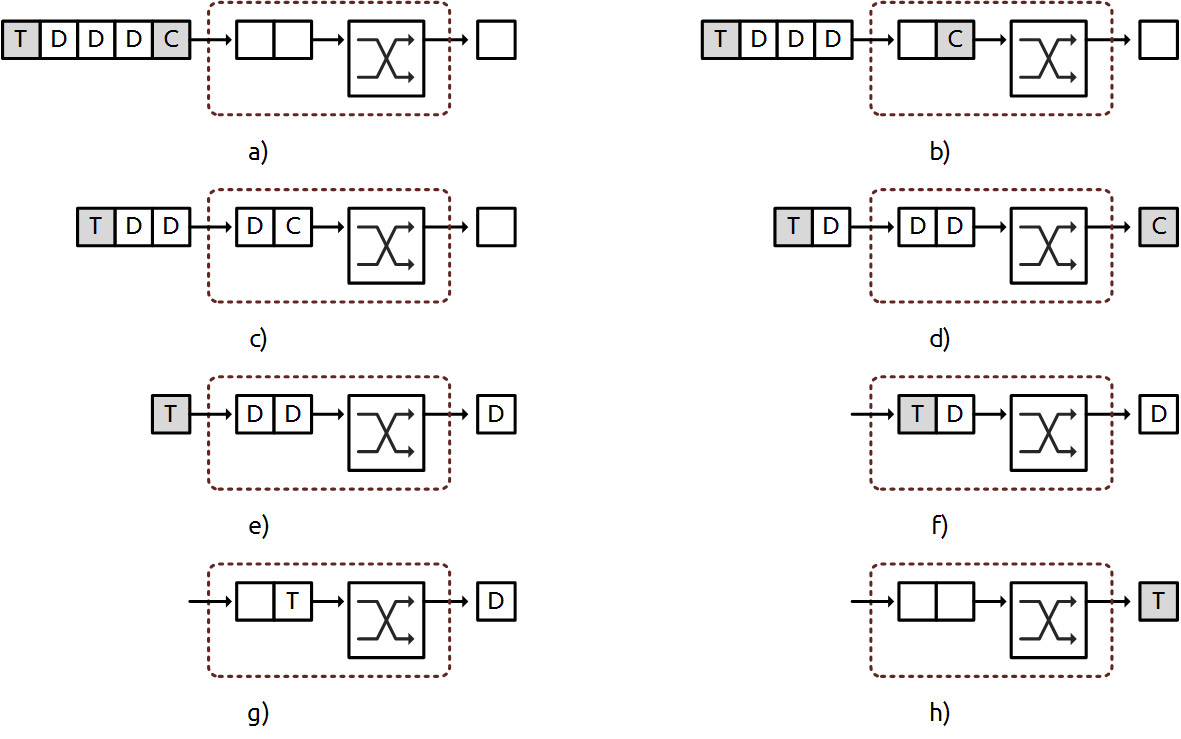
\includegraphics[width=\linewidth]{figures/ch1_wormhole.png}
	\caption
		{	
			Transferencia con control de flujo wormhole. Los flits que conforman el paquete presentan los siguientes identificadores: C (cabecera), D (datos o carga) y T (terminación).
			El concepto de transferencia es similar al control tipo cut-through, su única diferencia es la garantía de espacio en buffer requerido para continuar la transferencia de paquetes. El comportamiento de wormhole es exactamente igual al comportamiento de cut-through cuando este último tiene disponible el espacio de buffer en el siguiente nodo durante la llegada de un nuevo paquete.
		}
	\label{fig:ch1_wormhole}
\end{figure}

Virtual channels o canales virtuales\cite{chapter1:6663237, chapter1:Mello:2005:VCN:1081081.1081128}, es un mecanismo para incrementar el rendimiento de estrategias de control de flujo.  Este mecanismo recurre al uso de múltiples estructuras de almacenamiento temporal en cada puerto de entrada de un router, creando buffers alternativos para la recepción de paquetes. En caso de que un paquete almacenado no pueda continuar su camino, el router habilita un segundo buffer para la recepción de paquetes entrantes. Si un paquete almacenado en el buffer secundario del router cuenta con los recursos necesarios para abandonar el nodo de manera inmediata así lo hace. Esta técnica incrementa el rendimiento de la red al proveer un mecanismo para el salto de paquetes en espera por disponibilidad de recursos. Una desventaja en el uso de canales virtuales es el incremento en la complejidad de la lógica de control de cada router, ademas de un incremento de área necesaria para los buffers adicionales. La figura \ref{fig:ch1_vc} ejemplifica el uso de canales virtuales, en este escenario el paquete \textit{A} llega al router y es almacenado en el canal virtual número 1, figura \ref{fig:ch1_vc} (a,b). El paquete \textit{A} desea avanzar por el puerto de salida superior, sin embargo este se encuentra bloqueado por lo que \textit{A} debe de esperar para continuar su camino. Un segundo paquete se presenta a la entrada del router, este en respuesta habilita el canal virtual número 2 y empieza la recepción del paquete \textit{B}, figura \ref{fig:ch1_vc} (c). El puerto solicitado por \textit{B} se encuentra disponible, por lo que el router selecciona el canal virtual número 2 como el canal activo y empieza la transmisión del paquete \textit{B}, figura \ref{fig:ch1_vc} (d). Si no se encontraran canales virtuales en este router, el paquete \textit{B} tendría que esperar por el avance del paquete \textit{A}.   


\begin{figure}
	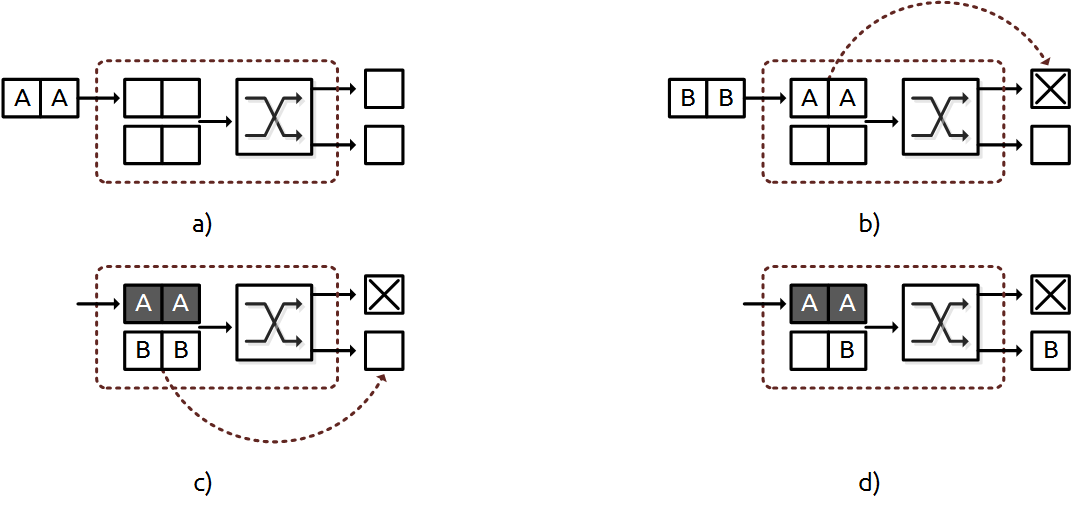
\includegraphics[width=\linewidth]{figures/ch1_vc.png}
	\caption
		{	
			Uso de canales virtuales. Un router con canales virtuales utiliza múltiples buffers, denominados canales virtuales, para evitar la congestión de la red debido a la espera de liberación de recursos.
		}
	\label{fig:ch1_vc}
\end{figure}

La principal diferencia entre los métodos con granularidades de paquete o flit, radica en el tamaño de medio de almacenamiento que requiere cada uno. En caso de utilizar un esquema basado en paquetes se requerirá un área mayor de silicio para la implementación de los buffers.

\subsection{Fuentes de consulta}

\textit{Reliability, Availability and Serviceability of Networks-on-Chip}\cite{chapter1:cota2011reliability} ofrece un resumen más amplio sobre los fundamentos de NoCs en su segundo capítulo. En el texto \textit{Interconnection Networks: An Engineering Approach}\cite{chapter1:Duato:2002:INE:572400} se aborda un amplio espectro de estructuras de interconexión desde buses hasta redes en-chip. \textit{Principles and Practices of Interconnection Networks}\cite{chapter1:Dally:2003:PPI:995703} es una referencia obligatoria para cualquier persona iniciando en el diseño de redes en-chip. Palesi \textit{et al.}\cite{chapter1:Palesi:2013:RAN:2556370} presentan una recopilación de algoritmos de encaminamiento específicos para redes en-chip.


\section{Modelo SPMD}\label{sec:modelo_spmd}

El modelo \textit{SPMD}\cite{chapter1:192215}(\textit{Single Program, Multiple Data}) es una técnica para la explotación de paralelismo en tareas de procesamiento. Dentro de la taxonomía de Flynn\cite{chapter1:Flynn:1972:COE:1952456.1952459} se clasifica como una subcategoría del grupo MIMD(\textit{Multiple Instructions, Multiple Data}). Bajo esta organización de procesamiento una misma tarea se ejecutará, sobre diferentes conjuntos de datos, en múltiples unidades de procesamiento de manera paralela. A diferencia del modelo SIMD(\textit{Single Instruction, Multiple Data}), SPMD utiliza múltiples procesadores independientes, los cuales cuentan con sus propias unidades de control. El uso de unidades de control independientes permite a arquitecturas SPMD el utilizar como unidades funcionales procesadores de propósito general, a diferencia de SIMD que requiere una arquitectura de procesador vectorial para implementar su modelo de ejecución paralela. Este modelo de procesamiento empata con arquitecturas MPSoC.


